\noindent Para determinar la distancia entre $r_1$ y $r_2$ hacemos uso de la siguiente expresión:

\begin{center}
	$\boxed{\delta(r_1;r_2) = \left|\overrightarrow{P_1P_2} \cdot \dfrac{\vec{u} \times \vec{v}}{|\vec{u} \times \vec{v}|} \right|}$
\end{center}

\noindent Realizamos los cálculos:
\begin{align*}
	\delta(r_1;r_2) & = \left|\overrightarrow{P_1P_2} \cdot \dfrac{\vec{u} \times \vec{v}}{|\vec{u} \times \vec{v}|} \right| \\
	\delta(r_1;r_2) & = \left|\dfrac{\overrightarrow{P_1P_2} \cdot \vec{u} \times \vec{v}}{|\vec{u} \times \vec{v}|} \right| \\
	\delta(r_1;r_2) & = \left|\dfrac{-8}{(-10, -17, 1)} \right|                                                              \\
	\delta(r_1;r_2) & = \left|\dfrac{-8}{\sqrt{(-10)^2 + (-17)^2 +  (1)^2}} \right|                                          \\
	\delta(r_1;r_2) & = \left|\dfrac{-8}{\sqrt{100 + 289 +  1}} \right|                                                      \\
	\delta(r_1;r_2) & = \left|\dfrac{-4}{195}\sqrt{390} \right|                                                              \\
	\delta(r_1;r_2) & = \dfrac{4}{195}\sqrt{390}                                                                             \\
	\delta(r_1;r_2) & \approx 0.405                                                                                          \\
\end{align*}
$\therefore$ \ La distancia entre las rectas $r_1$ y $r_2$ es \fcolorbox{black}{yellow}{$\approx 0.405$}.

\newpage
\noindent \textbf{Gráfica 23}:
\begin{center}
	\href{https://www.geogebra.org/3d/ghqqu7e7}{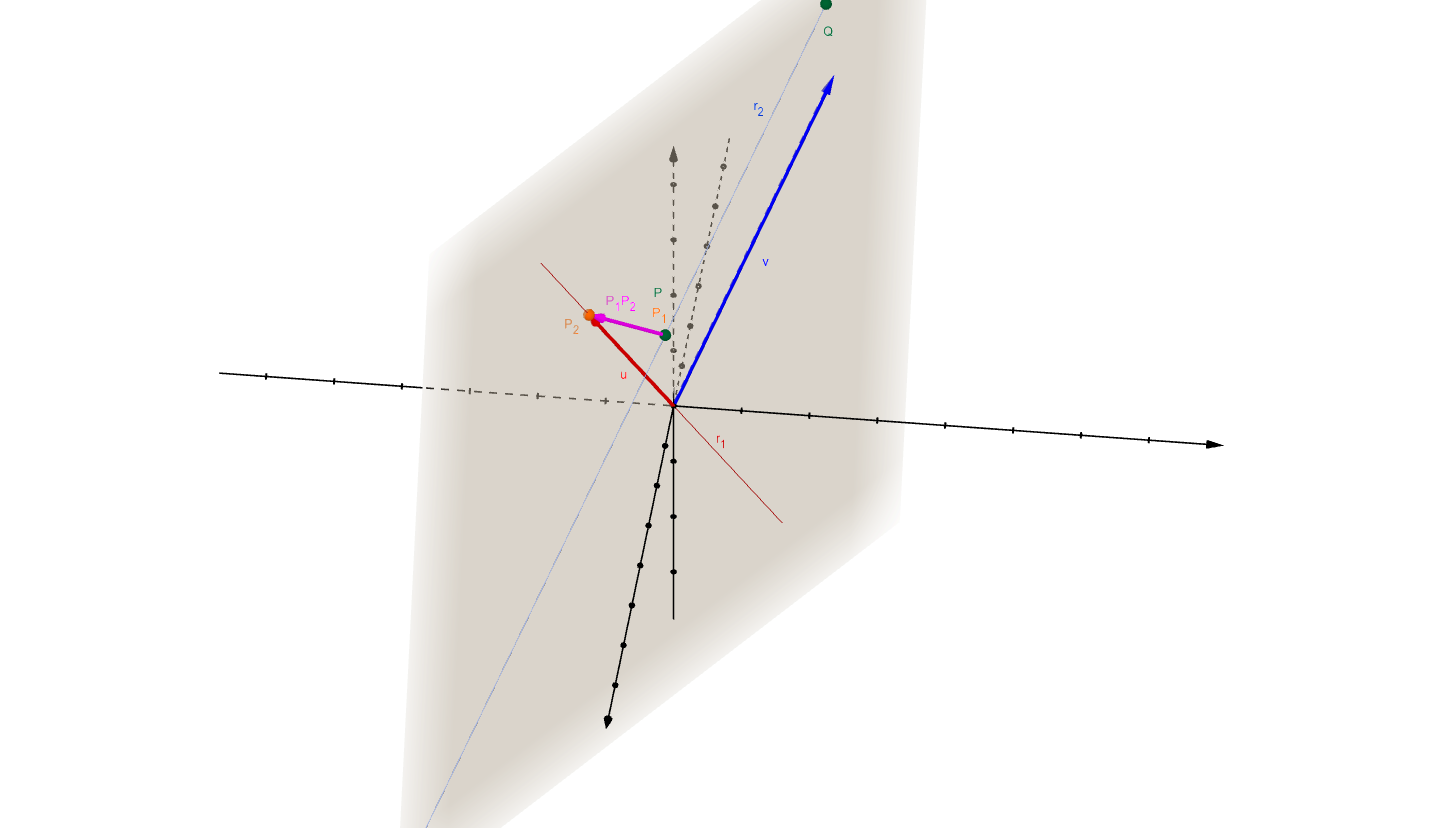
\includegraphics[width=15cm, scale=1]{TP-MATEMATICA-EJ23.png}}
\end{center}
